\documentclass[14pt, a4paper]{report}
\usepackage{mathtext}
\usepackage[T2A]{fontenc}
\usepackage[utf8]{inputenc}
\usepackage[russian]{babel}
\usepackage{multirow}
\usepackage{slashbox}
\usepackage{makecell}
\usepackage{graphicx}
\usepackage{physics}
\usepackage{amstext}
\usepackage{caption}
\usepackage{subcaption}

\renewcommand{\thesection}{\arabic{section}.}
\renewcommand{\thesubsection}{\arabic{section}.\arabic{subsection}.}

\title{\textbf{Отчет о выполнении лабораторной работы 2.3.1 "Получение и измерение вакуума"}}
\author{Калашников Михаил, Б03-205}
\date{}

\begin{document}
\maketitle

\textbf{Цель работы:}
измерение объемов форвакуумной и высоковакуумной частей установки; определение скорости откачки системы в стационарном режиме, а также по ухудшению и по улучшению вакуума
\newline

\textbf{В работе используются:}
\begin{itemize}
\item вакуумная установка;
\item маслянный манометр;
\item термопарный манометр;
\item ионизационный манометр;
\end{itemize}

\section{Теоретическая часть}

Вакуумом называют состояние газа при котором его давление меньше атмосферного ($P<P_0$). Различают следующие типы вакуума: низкий, когда средняя длина свободного пробега молекул газа значительно меньше характерного линейного размера рассматриваемого объёма, т.е. $\lambda<d$; средний, когда $\lambda\sim d$; высокий (или глубокий), когда $\lambda \gg d$ (рис. 1).

\begin{figure}[!ht]
\centering
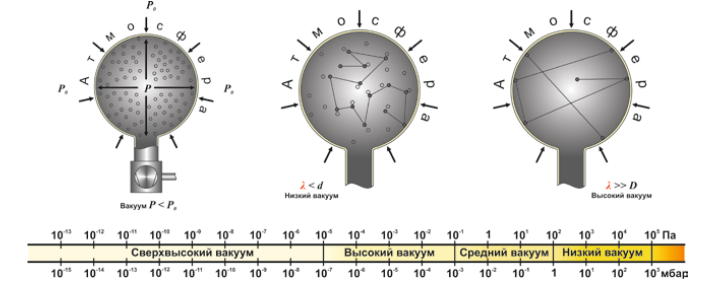
\includegraphics[scale=0.6]{terma5_02.png}
\caption{Понятие о вакууме}
\end{figure}

Запишем основное уравнение вакуумной техники, связывающее основные параметры вакуумной системы:
\[\frac{1}{S_0}=\frac{1}{S_н}+\frac{1}{U}\]
где $S_0$ -- эффективная скорость откачки камеры, $S_н$ -- быстродействие насоса, а $U$ -- пропускная спопособность вакуумпровода.

Определим время откачки. Пусть за время $\dd{t}$ давление в откачиваемом объеме $V_0$ снизилось на $\dd{P}$. Тогда за время $\dd{t}$ в трубку поступает $S_0P\dd{t}$ газа. С другой стороны это количество равно $-V_0\dd{P}$. Из этого равенства следует, что:
\[\frac{\dd{P}}{P}=-\frac{S_0}{V_0}\dd{t}\]

Количественной характеристикой течи является натекание:
\[Q_н=V\frac{P_к-P_н}{\Delta t}\]

Число Кнудсена определяется как
\[Kn=\frac{\lambda}{d}\]
где $\lambda$ -- длина свободного пробега молекул в газе, $d$ -- характерный линейный размер емкости.

\section{Экспериментальная установка}

\subsection{Общие сведения}

Экспериментальный стенд выполнен на основе компактного высоковакуумного откачного поста Edwards серии EXPT с пластинчато-роторным и турбомолекулярным насосами, вакууметров Edwards и вакуумных компонентов. Управление основными функциями откачного поста, контроль и запись параметров установки осуществляется блоком управления (БУ) через цифровой интерфейс RS-232 с помощью специального программного обеспечения TIC PC Monitor10. Схема экспериментального стенда и его внешний вид представлены на рис. 2-3.

\begin{figure}[!ht]
\centering
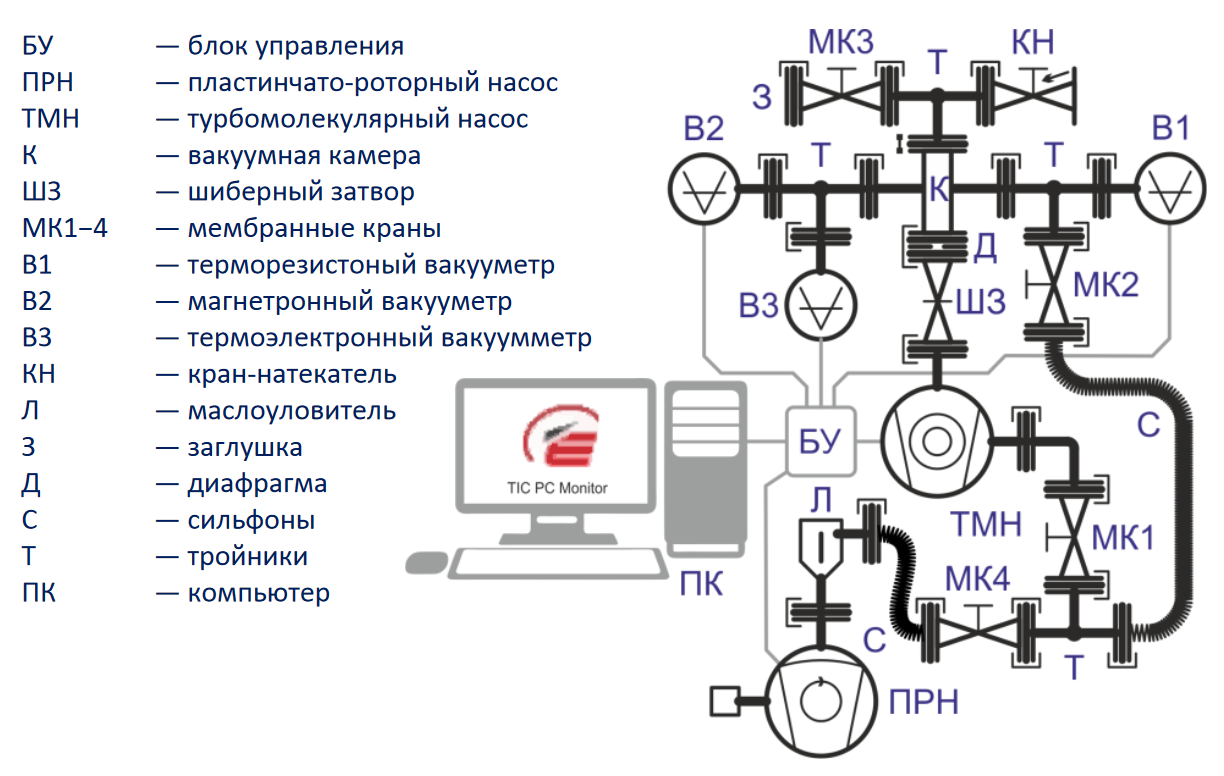
\includegraphics[scale=0.3]{terma5_00.png}
\caption{Схема экспериментальной установки}
\end{figure}

\begin{figure}[!ht]
\centering
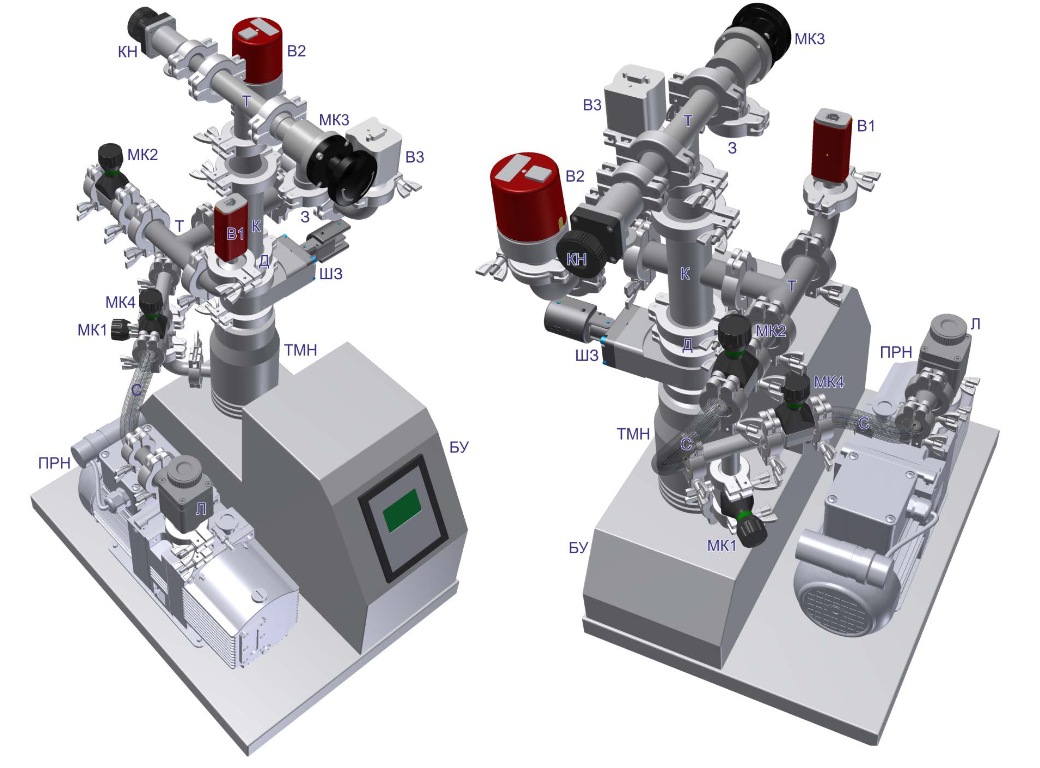
\includegraphics[scale=0.4]{terma5_01.png}
\caption{Внешний вид экспериментальной установки}
\end{figure}

Вакуумный пост Edwards EXPT выполнен на базе пластинчато-роторного форвакуумного насоса Е2М1.5 (ПРН) и турбомо-лекулярного насоса EXT70H (ТМН). Откачка вакуумной камеры (К) может происходить как двумя насосами (ТМН и ДН) через шиберный затвор (ШЗ) и мембранные краны 1 и 4 (МК1, МК4), так и только форвакуумным насосом (ПРН) по схеме «байпас», выполненной на основе вакуумных компонентов: сильфонов (С), мембранных кранов 2 и 4 (МК2, МК4), тройников (Т), переходников.

Для контроля и измерения давления в вакуумной камере используются цифровые вакууметры APG100-XM (В1) типа Пирани (терморезисторный) ($\varepsilon_P=15\%$), AIM-X (В2) инверсно-магнетронный ($\varepsilon_P=30\%$) и AIGX-S (В3) термоэлектронный (с накалённым катодом) ($\varepsilon_P=15\%$).

Контролированный напуск воздушной атмосферы в камеру осуществляется через кран-натекатель LV10K (КН) с регулируемым потоком. Дополнительный выход с краном 3 (МК3) закрыт заглушкой (З) и служит для присоединения дополнительного объёма в случае необходимости.

\subsection{Пластинчато-роторный насос}

В цилиндрическом корпусе (1) пластинчато-роторного насоса (рис. 4) со смещением эксцентрично размещен ротор (2), касающийся корпуса с одной стороны. Ротор снабжен пластинами (3), которые прижимаются к стенкам и скользят по внутренней поверхности. Газ, попадающий на вход (4) проталкивается пластинами и выталкивается из насоса через выпускной клапан (5).

\begin{figure}[!ht]
\centering
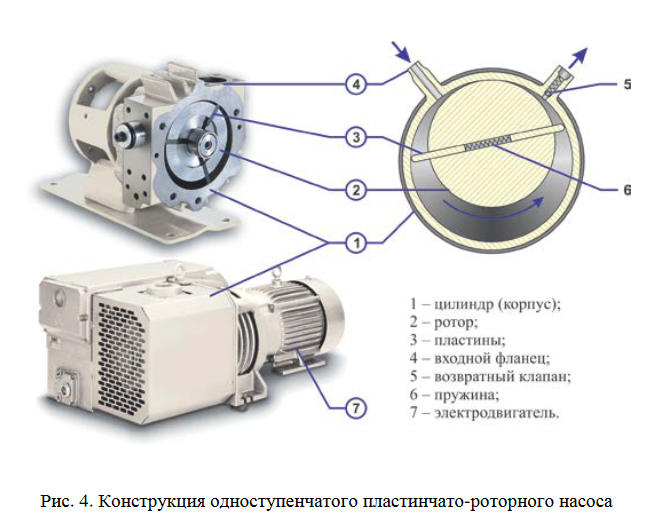
\includegraphics[scale=0.5]{terma5_03.png}
\caption{Конструкция одноступенчатого пластинчато-роторного насоса}
\end{figure}

\subsection{Турбомолекулярный насос}

Откачка в турбомолекулярном насосе (рис. 5) осуществляется за счет соударения частиц газа с быстродвижущимися турбинными лопатками дисков ротора (1) специальной геометрии, которые придают им дополнительный импульс в заданном направлении потока. Между дисками ротора находятся диски статора (2) с обратно обращенными лопатками, направляющие поток молекул на следующие диски турбины по оптимальной траектории, минимизируя обратный поток. Каждая пара пластин ротора-статора образует одну ступень. Насос состоит из нескольких ступеней расположенных последовательно, каждая последующая ступень имеет меньшие геометрические размеры, что при постоянном потоке газа приводит к постепенному повышению давления до выпускного форвакуумного. Скорость вращения ротора современных турбомолекулярных насосов достигает нескольких десятков тысяч оборотов в минуту.

\begin{figure}[!ht]
\centering
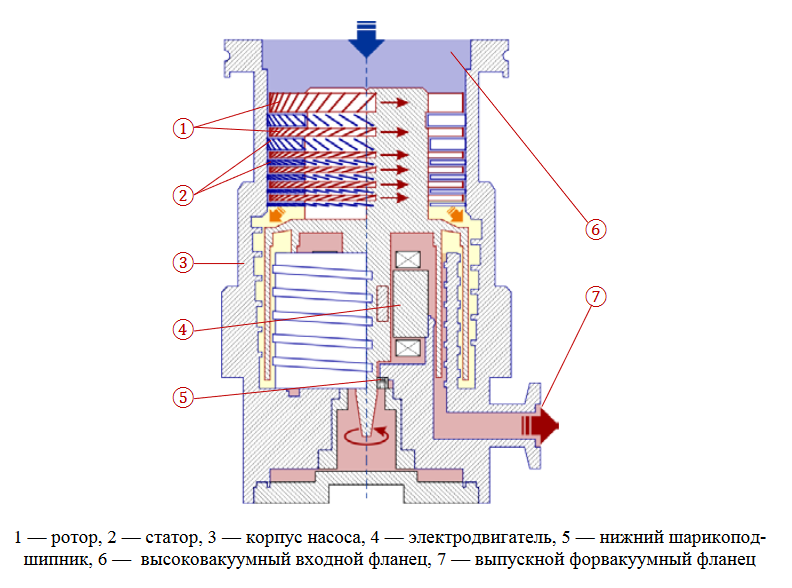
\includegraphics[scale=0.5]{terma5_04.png}
\caption{Конструкция турбомолекулярного насоса}
\end{figure}

\subsection{Терморезисторный вакуумметр (Пирани)}

Принцип действия тепловых манометров основан на зависимости теплопроводности газа от давления. Чувствительным элементом терморезисторного датчика (рис. 6) является тонкая металлическая нить накала, помещенная в атмосферу откачиваемого газа. Сопротивление нити зависит от её температуры. Нить включена в одно из плеч мостовой схемы и разогрета до нескольких сотен градусов пропускаемым по ней током. Джоулево тепло, выделяемое нитью, отводится в основном через газовую среду со скоростью, зависящей от коэффициента теплопроводности.

\begin{figure}[!ht]
\centering
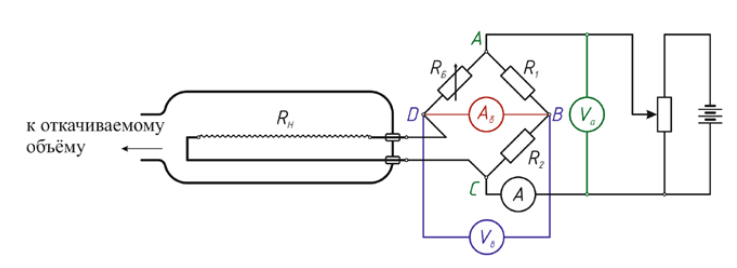
\includegraphics[scale=0.5]{terma5_05.png}
\caption{Принципиальная схема терморезисторного вакуумметра (Пирани)}
\end{figure}

\subsection{Магнетронный вакуумметр (с холодным катодом)}

Измерительный объём магнетронного датчика (рис. 7) находится между катодом и анодом, между которыми приложено напряжение, а также помещен в постоянное магнитное поле. Случайным образом возникшие вблизи катода электроны будут двигаться к аноду под действием скрещенных электромагнитных полей по удлиненной траектории. При этом повышается вероятность соударения электронов с молекулами откачиваемого газа и их ионизация. Образовавшиеся ионы ускоряются в электрическом поле анодно-катодного промежутка и выбивают из материала катода вторичные электроны, которые также ионизируют газ, двигаясь к аноду по сложной циклической траектории. В результате описанного процесса возникает электрический разряд, ток которого в достаточно широком диапазоне зависит от давления.

\begin{figure}[!ht]
\centering
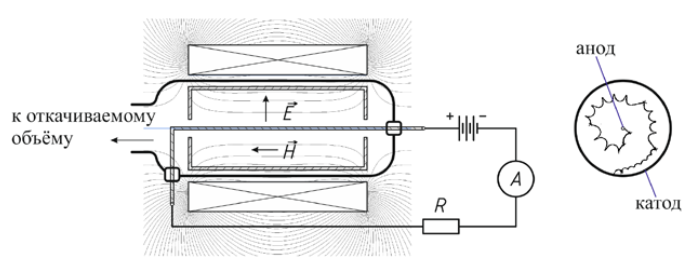
\includegraphics[scale=0.5]{terma5_06.png}
\caption{Принципиальная схема инверсно-магнетронного вакуумметра и траектории электронов в них}
\end{figure}

\subsection{Термоэлектронный вакуумметр (с накалённым катодом)}

Катодом термоэлектронного вакуумметра является накаливаемаянить (1) (рис. 8). Эмитируемые накаленным катодом электроны под действием ускоряющего электрического поля устремляются по направлению к аноду (2), создавая в его цепи (5) электронный ток. Анод, как правило, выполнен в виде спирали или сетки с большим шагом, поэтому значительная часть электронов проходит между витками анода и тормозится полем коллектора 3, имеющего по отношению к катоду отрицательный потенциал. Не дойдя до коллектора ионов, электроны останавливаются и начинают движение обратно к аноду-сетке. Снова значительная часть электронов проходит между витками анода и тормозится уже полем катода. Каждый электрон может сделать несколько таких колебаний, прежде чем попасть на сетку. Времени жизни электронов в откачиваемом объеме достаточно, чтобы ионизировать значительную часть находящегося в датчике газа. Ионы притягиваются полем коллектора, рекомбинируют на его поверхности, создавая в цепи коллектора 6 ионный ток. Ионный ток в цепи коллектора пропорционален плотности газа и служит мерой давления.

\begin{figure}[!ht]
\centering
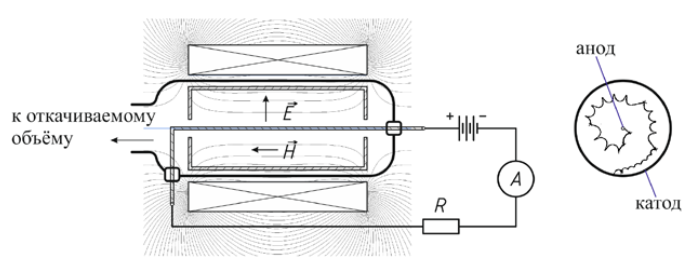
\includegraphics[scale=0.5]{terma5_06.png}
\caption{Принципиальная схема термоэлектронного вакуумметра}
\end{figure}

\section{Проведение эксперимента}

\begin{enumerate}

\item Зафиксируем температуру и атмосферное давление в лаборатории:

\[T_0=297,9\pm0,1\ К,\quad P_0=98,77\pm0,01\ кПа\]

\item Выровняем давление во всей установке, открыв все краны и шиберный затвор. Впустим в установку атмосферный воздух.

\item Подготовим установку к форвакуумной откачке, перекрыв доступ атмосферы в установку, закрыв кран МК3 и шиберный затвор ШЗ.

\item Подключим установку к компьютеру и настроим программу так, чтобы показания вакууметров записывались в файл каждые 2 секунды.

\item Включим ПРН и откачаем систему до предельного значения.

\item Соблюдая правила вакуумной гигиены, присоединим к установке сильфон с воздухом при атмосферном давлении.

\item Закроем кран МК2. Выровняем давление в сильфоне и вакуумной камере медленным поворотом крана МК3.

\item Закроем краны МК1 и МК4. Выровняем давление в вакуумной камере и форвакуумной магистрали установки плавным поворотом крана МК2.

\item Теперь же аккуратно откроем кран МК1, чтобы выровнять давление во всей установке, включая объем насоса ТМН.

\item Заполним установку воздухом при атмосферном давлении с помощью крана КН, предварительно отключив ПРН.

\item Изолируем установку от атмосферы, закрым кран КН.

\item Повторим пункты 5-11 еще один раз.

\item Теперь проведем измерение скорости откачки турбомолекулярного насоса. Отсоединим сильфон от установки, соблюдая правила вакуумной гигиены.

\item Откачаем установку форвакуумным насосом.

\item Откроем шиберный затвор и закроем кран МК2. Запустин насос ТМН. Таким образом он откачает воздух из объема всей установки. Откачаем установку до предельного давления, определяемого динамикой показаний манометров В2 и В3.

\item Проведем обезгаживаение манометра В3.

\item Определим уровень течей, изолировав вакуумную камеру перекрытием шибера ШЗ. Дождавшись момента, когда давление достигнет $10^{-3}\ Па$, откроем шибер.

\item Повторим предыдущий пункт еще два раза.

\end{enumerate}

\section{Обработка данных}

\begin{enumerate}

\item Перенесем данные из файла, содержащего измерения, на компьютер.

\item Зная объем $V_0$ воздуха в сильфоне, находящегося там под атмосферным давлением $P_0$, найдем по закону Бойля-Мариотта полный объём установки $V$, объем высоковакуумной части $V_1$, форвакуумной магистраи $V_2$, и объем насоса ТМН $V_3$.
\[V_0+V_1=V_0\frac{P_1}{P_0}\]
\[V_0+V_1+V_2=(V_0+V_1)\frac{P_2}{P_1}\]
\[V_0+V_1+V_2+V_3=(V_0+V_1+V_2)\frac{P_3}{P_2}\]

Давления $P_1-P_3$ найдем из полученных данных, как среднее значение давления перед пропусканием воздуха в следующую часть установки.

\item Теперь определим эффективную скорость откачки форвакуумным насосом. Будем делать это в диапазоне от давлений от $10^{2}\ Па$ до $10^{4}\ Па$, так как в этом диапазоне скорость откачки почти постоянна. Построим по отобранным точкам зависимость $\ln P$ от $t$. Получим прямую с коэффициентом наклона $k$. Отсюда скорость откачки:
\[\ln\frac{P}{P_0}=-\frac{S_1}{V}t=kt,\quad S_1=-kV\]

\item Повторим предыдущий пункт для определения скорости откачки турбомолекулярного насоса в диапазоне от $10^{-3}\ Па$ до $10^{-1}\ Па$. Отдельно посчитаем скорость для измерений проведенных с помощью разных манометров.

\[\ln\frac{P}{P_0}=-\frac{S_2}{V}t=kt,\quad S_{21}=-k_1V,\quad S_{22}=-k_2V\]

\item Рассчитаем натекание воздуха в установку. Построим зависимость давления от времени после закрытия шиберного затвора. Проведем через точки прямую. Тогда коэффициент наклона $k$ равен $\dv{P}{t}$. Отсюда найдем величину натекания:
\[Q_н=V_1\dv{P}{t}=kV_1\]
Усредним величину по всем проведенным измерениям для обоих манометров.

\item Оценим число Кнудсена:
\[Kn=\frac{\lambda}{L}=\frac{1}{\sigma nL}=\frac{kT}{4\pi r^2 PL}\]
где $r=200\ пм$ -- средний радиус молекулы в воздухе. 

\end{enumerate}

\section{Расчет погрешностей}

Найдем погрешность определения объемов установки.
\[\varepsilon_{V_0+V_1}=\sqrt{\varepsilon_{P_0}^2+\varepsilon_P^2}\approx\varepsilon_P=15,0\%\]
\[\varepsilon_{V_0+V_1+V_2}=\sqrt{\varepsilon_{V_0+V_1}^2+2\varepsilon_P^2}=\sqrt{3}\varepsilon_P=26,0\%\]
\[\varepsilon_{V_0+V_1+V_2+V_3}=\sqrt{\varepsilon_{V_0+V_1+V_2}^2+2\varepsilon_{P}^2}=\sqrt{5}\varepsilon_P=33,5\%\]

Пренебрегая $\varepsilon_{V_0}$, получим, что:
\[V_1=650\pm100\ мл,\quad V_1+V_2=830\pm170\ мл,\quad V=1240\pm420\ мл\]

Теперь посчитаем погрешность скорости откачки:
\[\varepsilon_{S_i}=\sqrt{\varepsilon_{k_i}^2+\varepsilon_V^2}=\sqrt{\varepsilon_{k_i}^2+5\varepsilon_P^2}=33,8\%\]
\[S_1=1,2\pm0,4\ \frac{м^3}{ч}\]
\[\varepsilon_{S_{21}}=69,3\%, \quad \varepsilon_{S_{22}}=44,3\%\]
\[S_{21}=1,6\pm1,1\ \frac{мл}{с},\quad S_{22}=1,7\pm0,8\ \frac{мл}{с}\]

Погрешность натекания:
\[\varepsilon_{Q_{нi}}=\sqrt{\varepsilon_{k_i}^2+\varepsilon_{V_1}^2}=\sqrt{\varepsilon_{k_i}^2+\varepsilon_P^2}\]
\[\varepsilon_{Q_{н1}}=16,3\%,\quad \varepsilon_{Q_{н2}}=15,4\%\]
\[Q_{н1}=1,18\pm0,16\ \frac{мл\cdot Па}{с},\quad Q_{н2}=0,97\pm0,15\ \frac{мл\cdot Па}{с}\]

Оценим погрешность числа Кнудсена по формуле (результаты занесем в таблицу 1):
\[\varepsilon_{Kn}=\sqrt{\varepsilon_T^2+\varepsilon_P^2+\varepsilon_L^2}\]

\section{Вывод}

В ходе работы получилось определить скорость откачки насоса ПРН. Она практически совпала с табличной, равной $1.8\ м^3/ч$. Однако скорость откачки турбомолекулярного насоса оказалась далека от настоящего значения, примерно равного $50\ л/c$. Очевидно, что полученное значение неверно, так как так при такой скорости откачки не получилось бы поддерживать измеряемое давление.

Полученные числа Кнудсена наглядно демонстрируют степень разреженности газа при откачке разными насосами.

\section{Приложения}

\begin{table}[!ht]
\makebox[\textwidth][c] {
\centering
\begin{tabular}{| c | c | c | c | c |}
\hline
\backslashbox{Насос}{Объем} & \makecell{$V_0$ \\ $(L=25\pm5\ мм)$} &  \makecell{$V_1$ \\ $(L=40\pm5\ мм)$} &  \makecell{$V_2$ \\ $(L=16\pm5\ мм)$} &  \makecell{$V_3$ \\ $(L=94\pm5\ мм)$} \\
\hline
\makecell{ПРН \\  ($P=20\ Па$)} & $0,016\pm0,004$ & $0,010\pm0,002$ & $0,026\pm0,009$ & $0,0044\pm0,0007$ \\
\hline
\makecell{ТМН\\ ($P=1\ мПа$)} & - & $204\pm40$ & $510\pm180$ & $87\pm14$ \\
\hline
\end{tabular}
}
\caption{Зависимость числа Кнудсена в различных частях установки при работе каждого из насосов}
\end{table}

\begin{figure}[!ht]
\centering
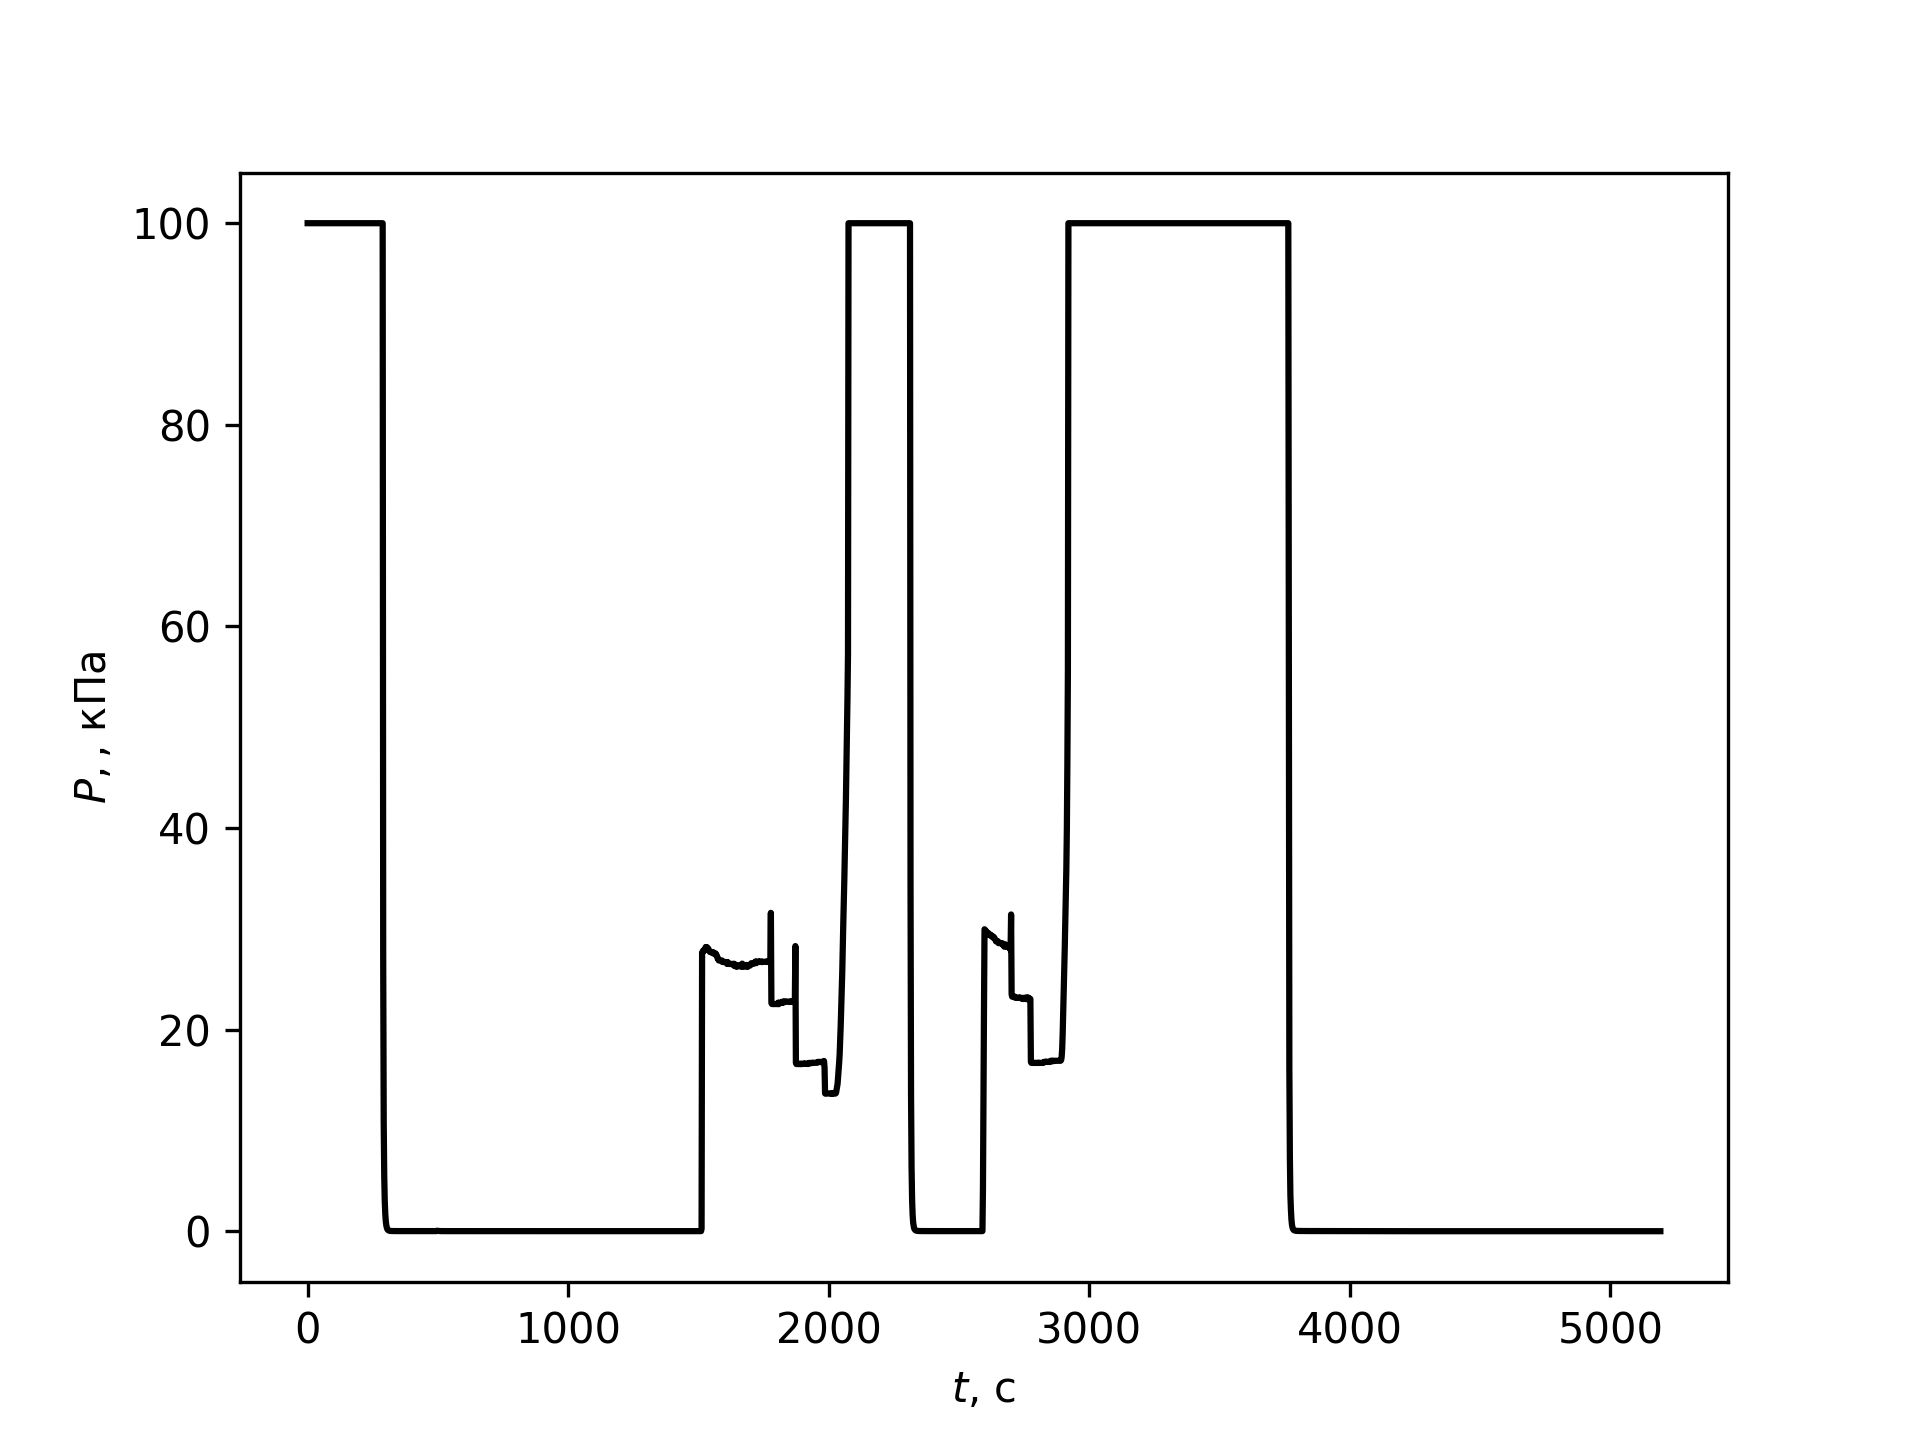
\includegraphics[scale=0.5]{terma5_1.png}
\caption{Показания манометра В1 за все время проведения работы}
\end{figure}

\begin{figure}
	\centering
	\begin{subfigure}{.5\textwidth}
		\centering
		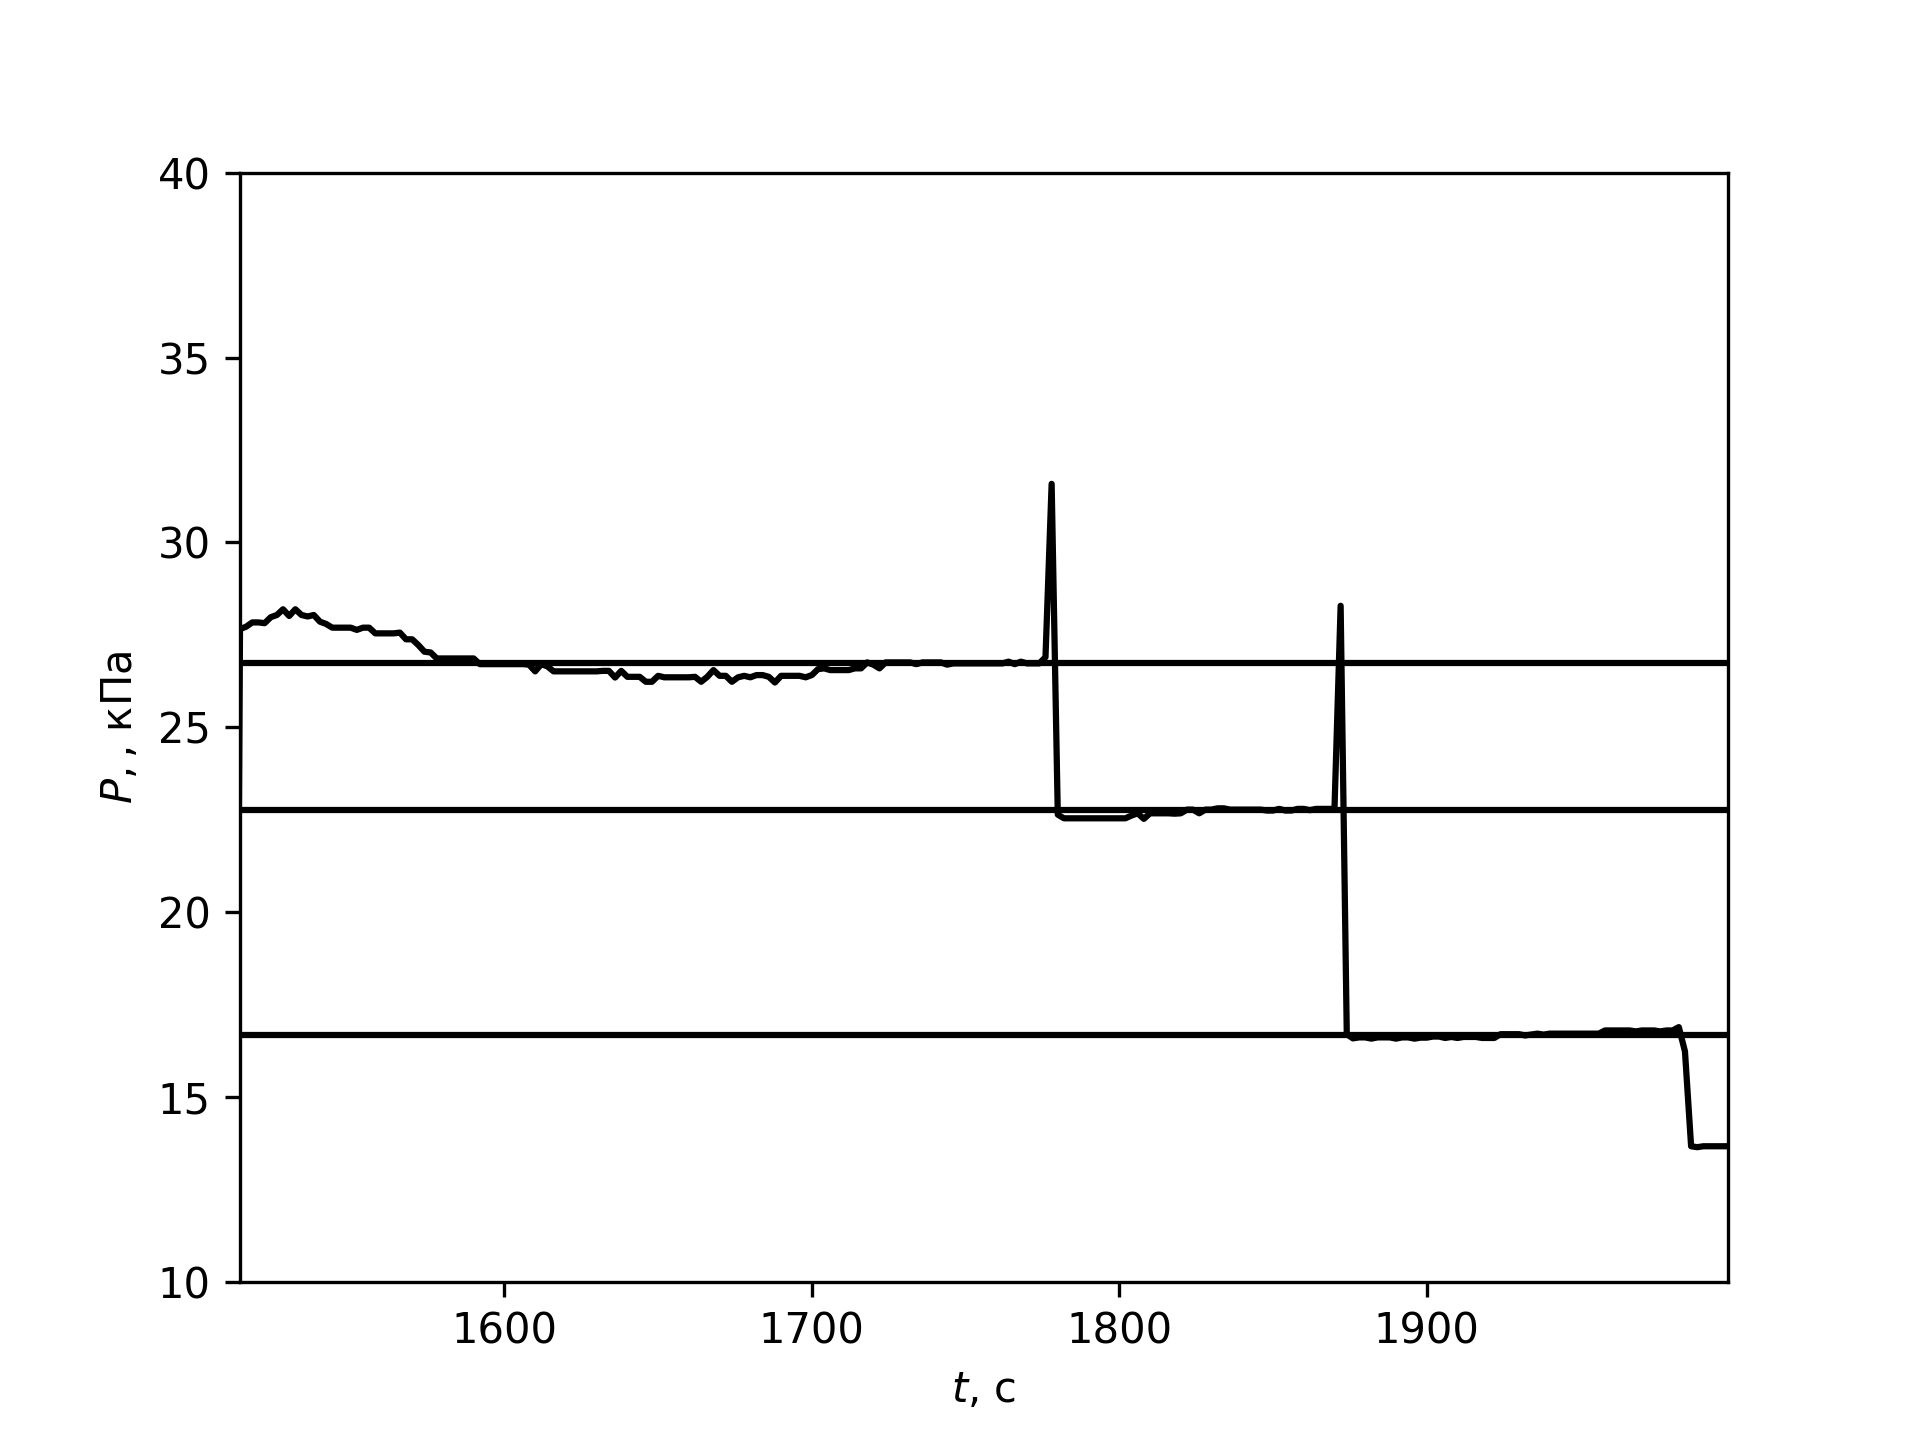
\includegraphics[width=\linewidth]{terma5_2.png}
	\end{subfigure}%
	\begin{subfigure}{.5\textwidth}
		\centering
		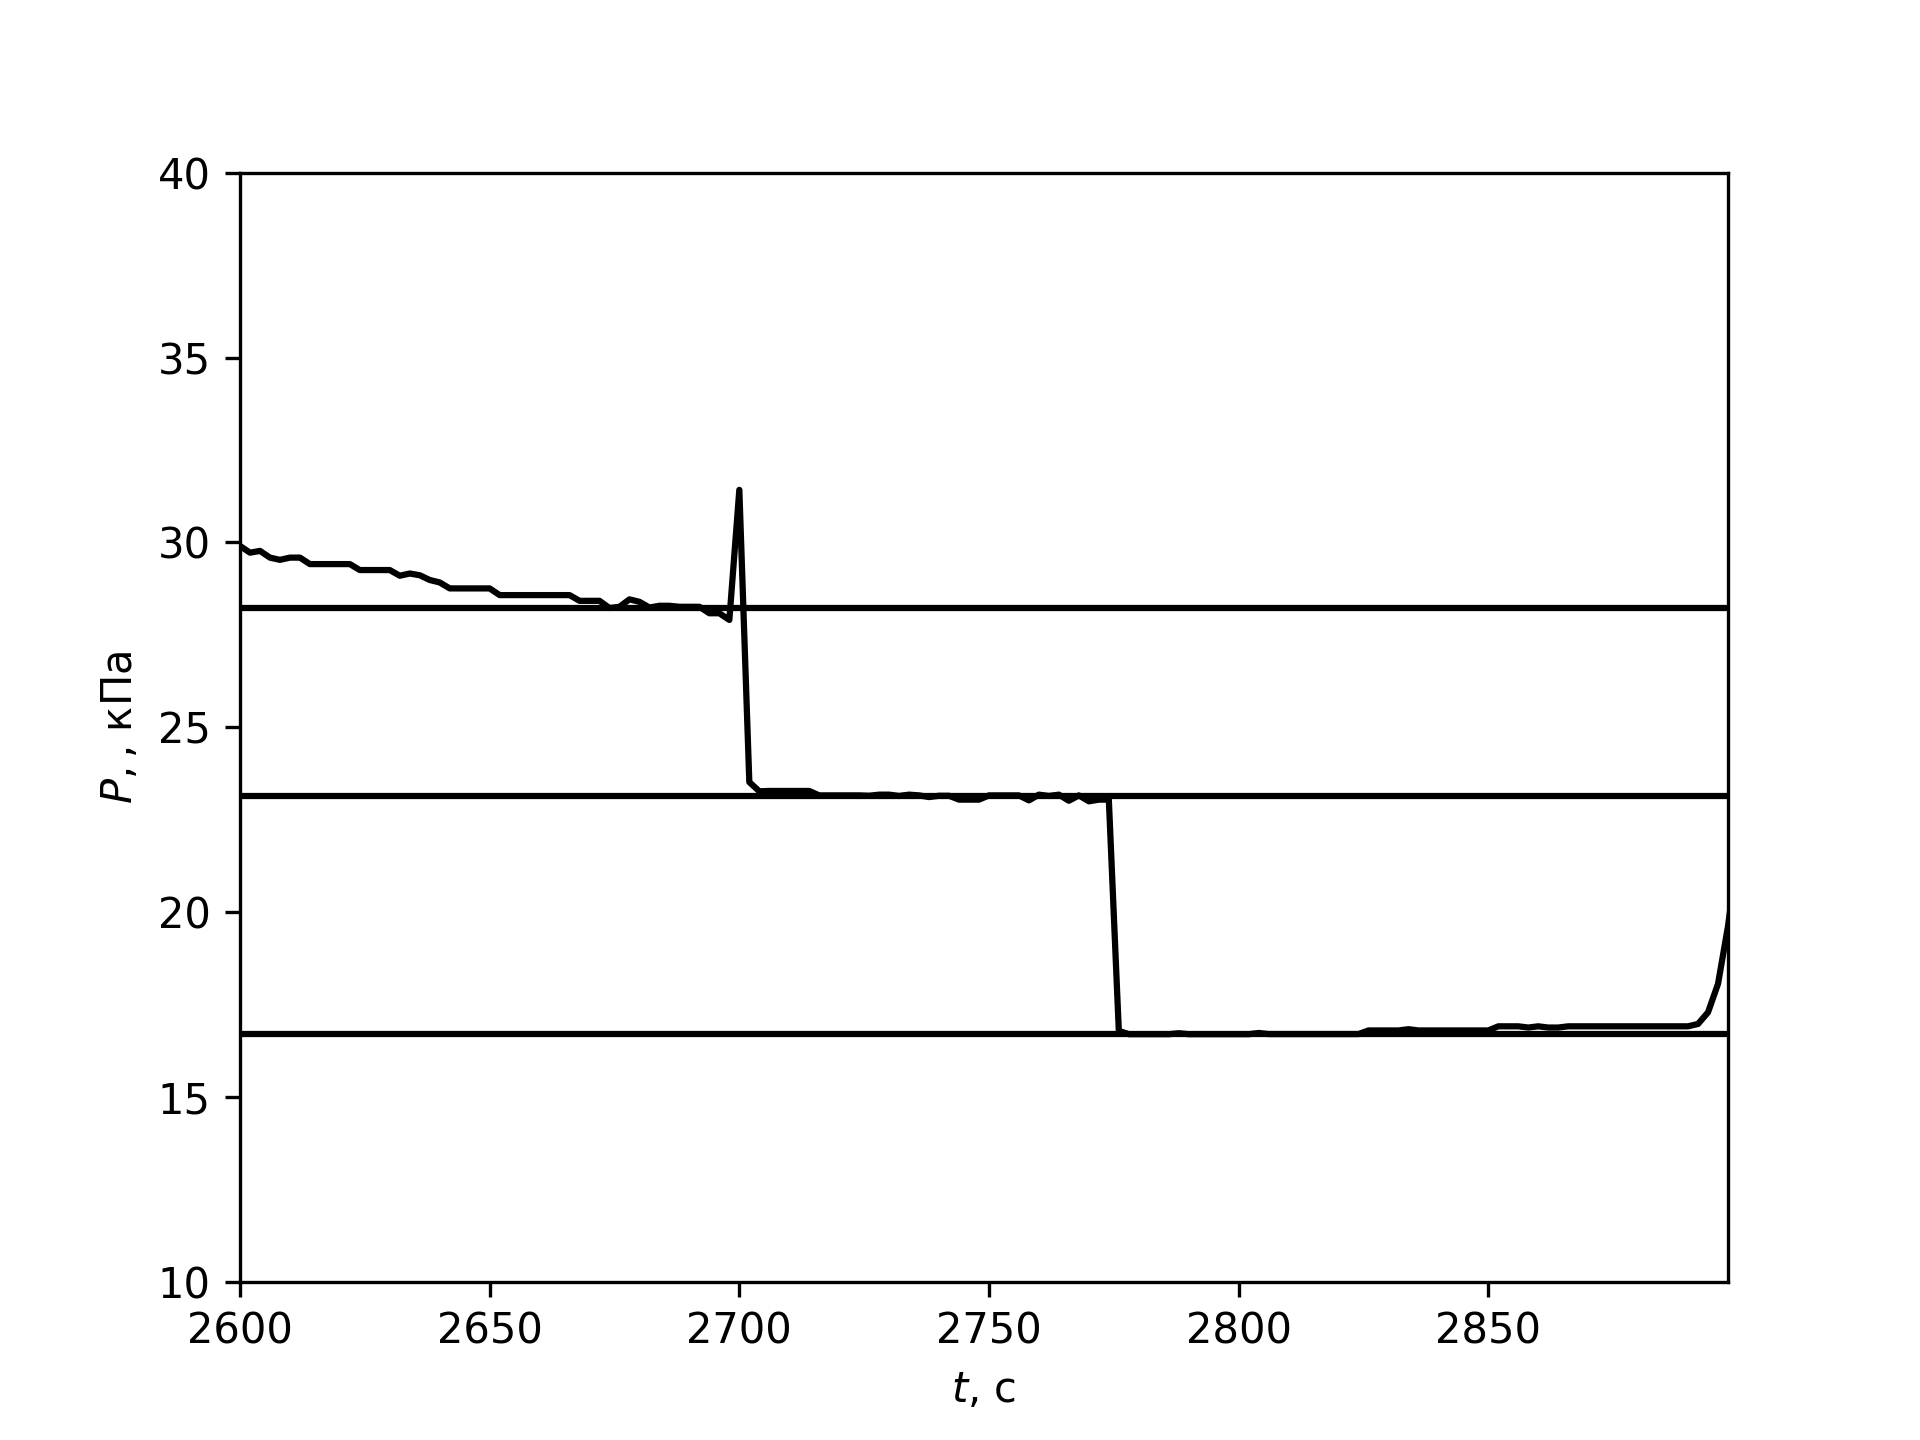
\includegraphics[width=\linewidth]{terma5_3.png}
	\end{subfigure}
	\caption{Показания манометра В1 при измерении объемов установки}
\end{figure}

\begin{figure}[!ht]
\centering
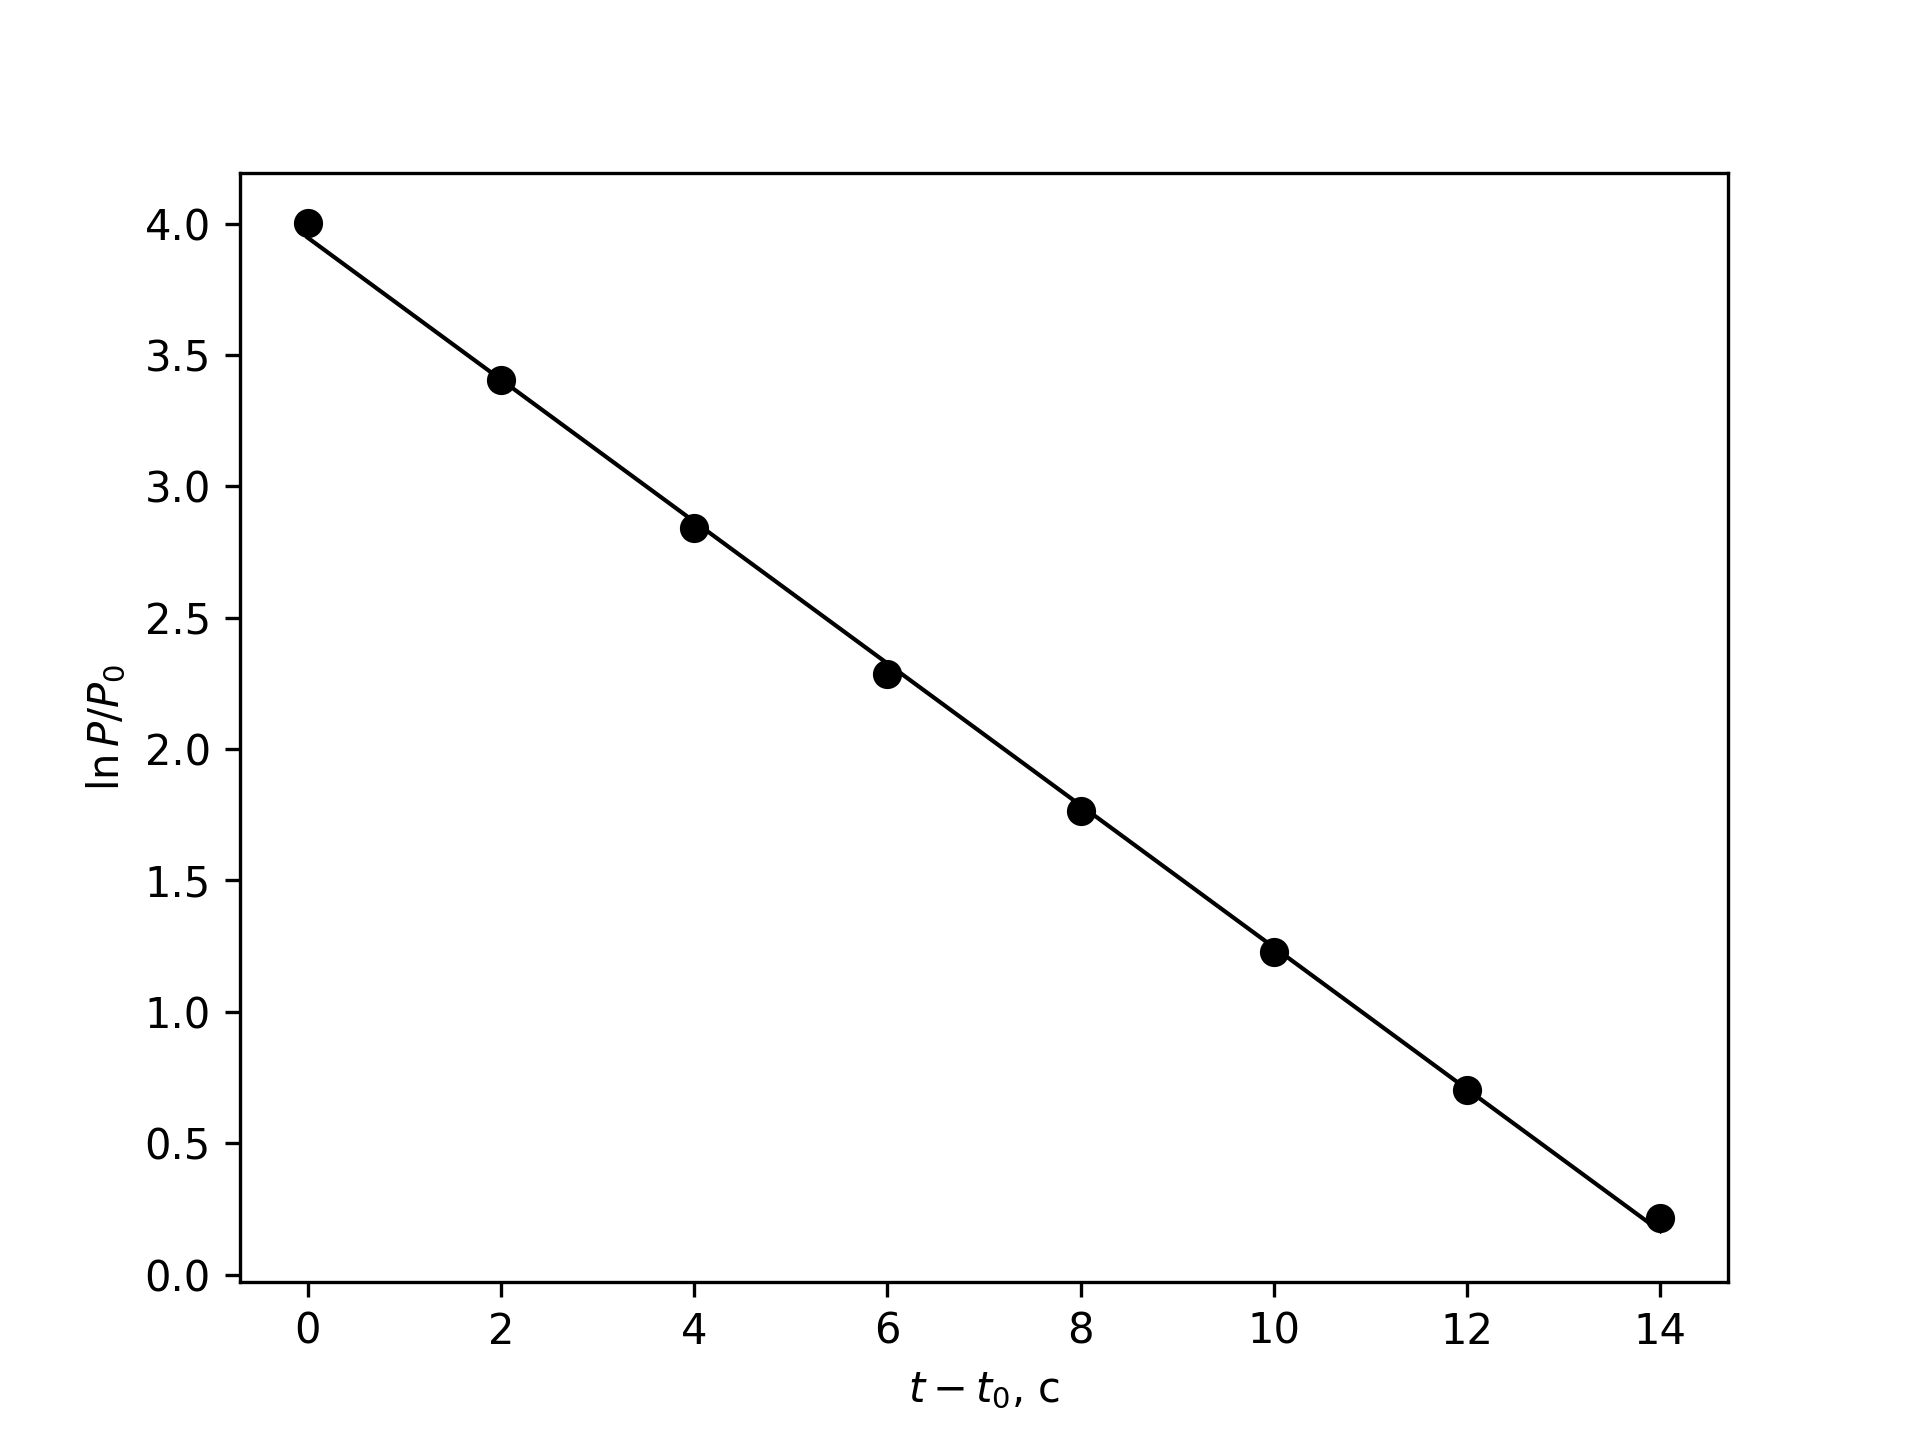
\includegraphics[scale=0.5]{terma5_4.png}
\caption{Зависимость $\ln P/P_0$ от $t-t_0$ при откачке насосом ПРН ($P_0=100\ Па$, $t_0$ -- время начала данной части работы). Показания манометра В1}
\end{figure}

\begin{figure}[!ht]
\centering
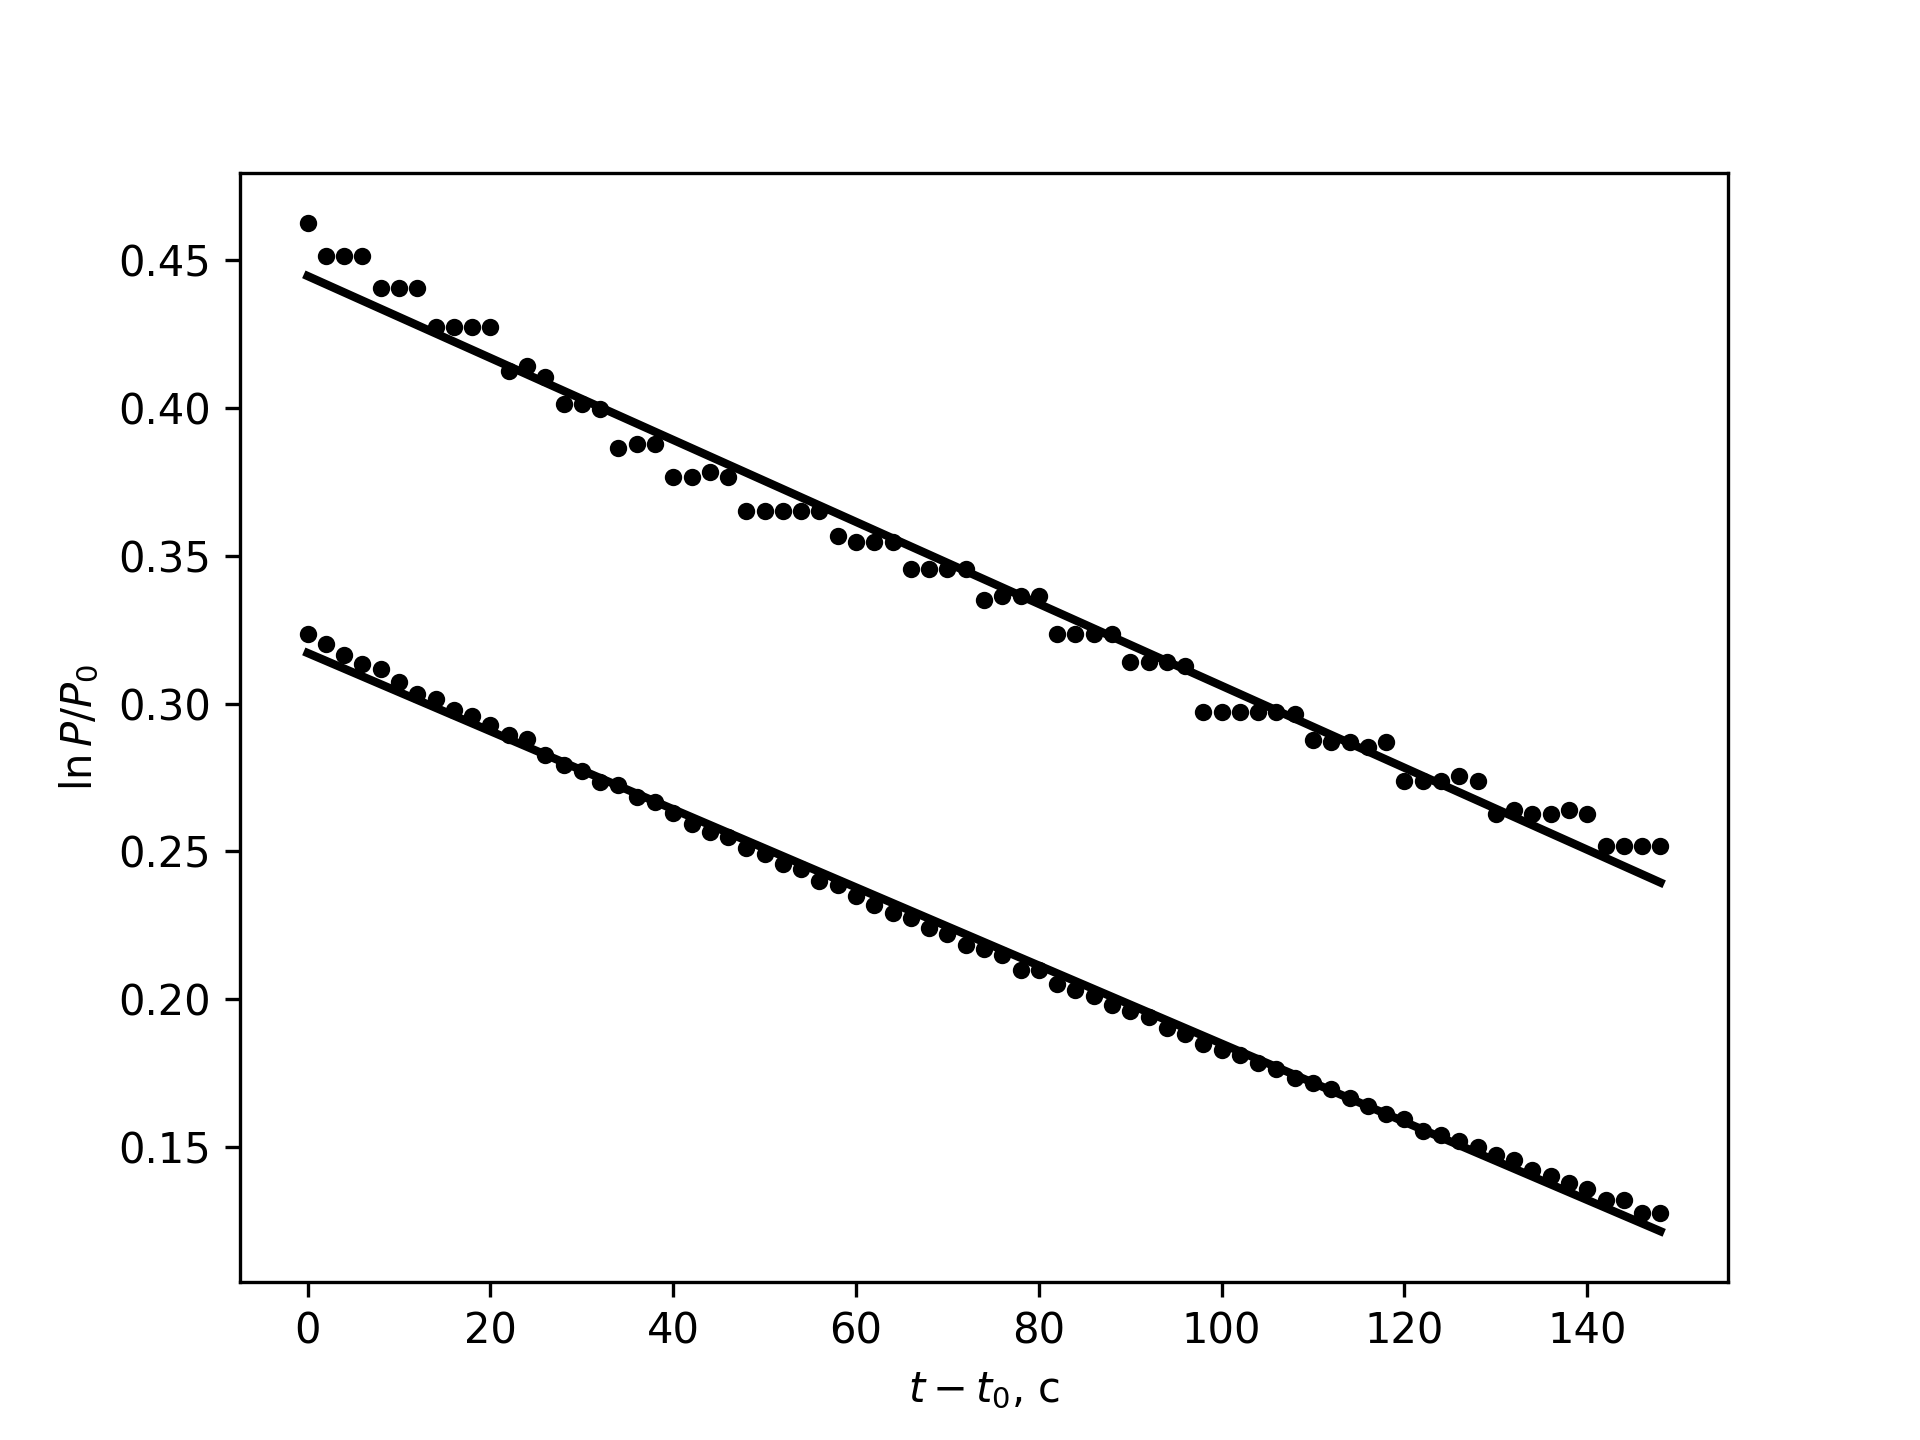
\includegraphics[scale=0.7]{terma5_5.png}
\caption{Зависимость $\ln P/P_0$ от $t-t_0$ при откачке насосом ТМН. ($P_0=1\ мПа$, $t_0$ -- время начала данной части работы). Показания манометров В2 (снизу) и В3 (сверху)}
\end{figure}

\begin{figure}[!ht]
\centering
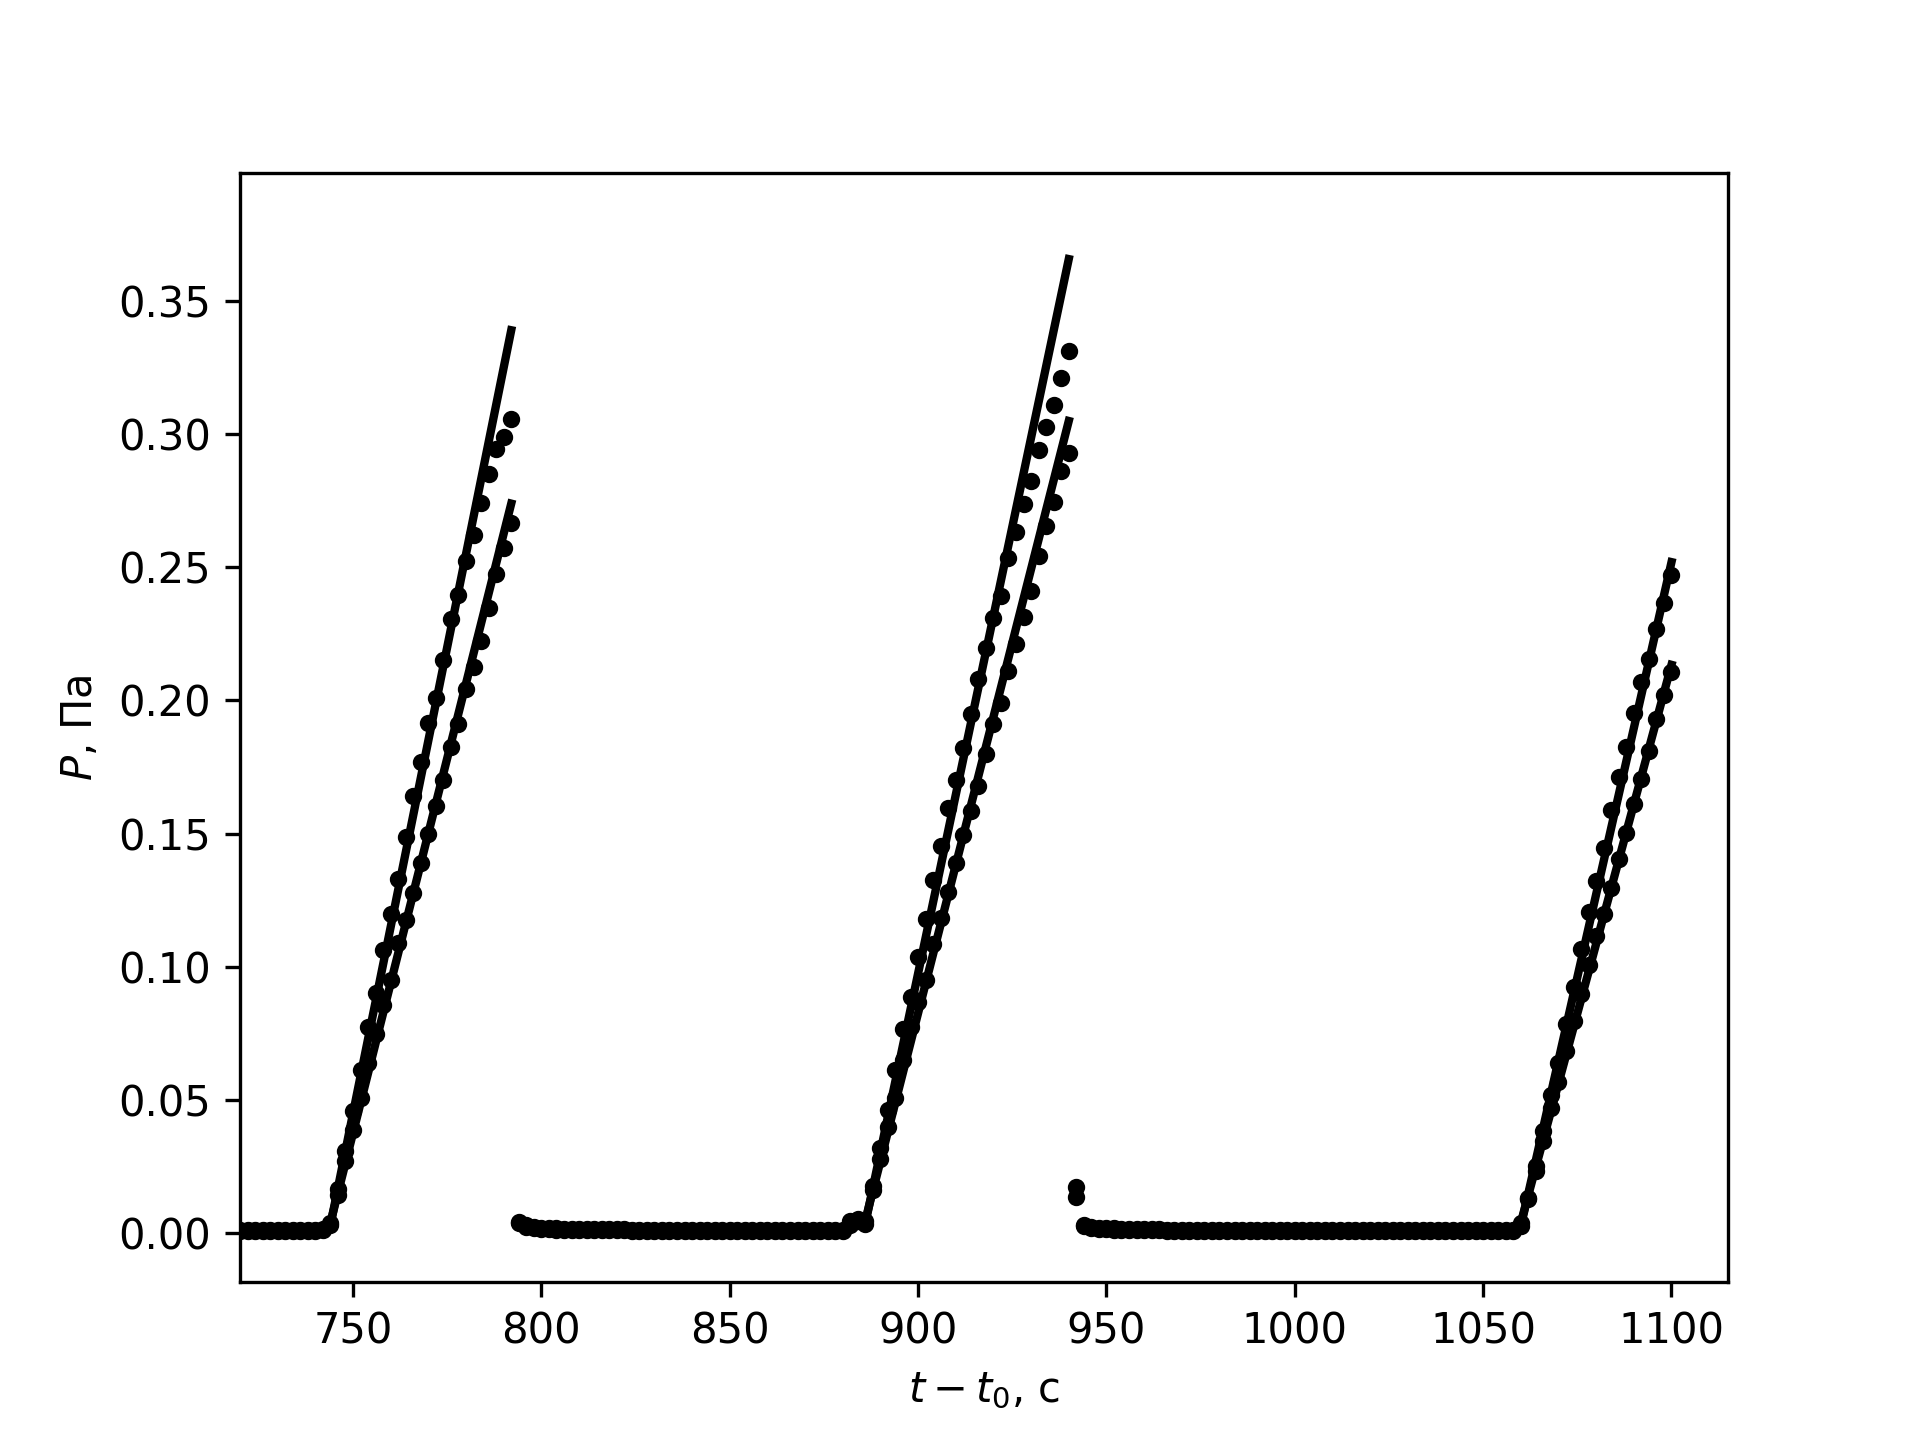
\includegraphics[scale=0.7]{terma5_6.png}
\caption{Три повторных измерения повышения давления в установке из-за течей ($t_0$ -- время начала данной части работы). Показания манометров В2 (сверху) и В3 (снизу)}
\end{figure}

\end{document}